% Template per generare 

\documentclass[a4paper,11pt]{article}
\usepackage{lmodern}
\renewcommand*\familydefault{\sfdefault}
\usepackage{sfmath}
\usepackage[utf8]{inputenc}
\usepackage[T1]{fontenc}
\usepackage[italian]{babel}
\usepackage{indentfirst}
\usepackage{graphicx}
\usepackage{tikz}
\usepackage{listings}
\newcommand*\circled[1]{\tikz[baseline=(char.base)]{
		\node[shape=circle,draw,inner sep=2pt] (char) {#1};}}
\usepackage{enumitem}
% \usepackage[group-separator={\,}]{siunitx}
\usepackage[left=2cm, right=2cm, bottom=3cm]{geometry}
\frenchspacing

\newcommand{\num}[1]{#1}

% Macro varie...
\newcommand{\file}[1]{\texttt{#1}}
\renewcommand{\arraystretch}{1.3}
\newcommand{\esempio}[2]{
\noindent\begin{minipage}{\textwidth}
\begin{tabular}{|p{8cm}|p{8cm}|}
	\hline
      \textbf{\file{input (da stdin)}} & \textbf{\file{output (su stdout)}}\\
	\hline
	\tt \small #1 &
	\tt \small #2 \\
	\hline
\end{tabular}
\end{minipage}
}

% Dati del task
\newcommand{\gara}{Esame Algoritmi 2018-06-18}
\newcommand{\nome}{Trascodifica di alberi ordinati riportando i figli o la discendenza}
\newcommand{\nomebreve}{tree\_transcode}

\begin{document}
% Intestazione
\noindent{\Large \gara}
\vspace{0.5cm}

\noindent{\Huge \textbf \nome~(\texttt{\nomebreve})}

% Descrizione del task
\section*{Descrizione del problema}

Un \emph{albero ordinato} consta di un \emph{nodo radice} e di una sequenza finita (eventualmente vuota) di \emph{figli} della radice, che sono a loro volta alberi ordinati. La figura offre due rappresentazioni dello stesso albero, nella prima su ogni nodo viene riportato il numero di figli di quel nodo, nella seconda, su ogni nodo viene riportato il numero dei suoi discendenti (incluso il nodo stesso). Per convenzione, la radice viene disegnata in cima (cio\`e al contrario rispetto agli alberi veri).

\begin{figure}[h!]
  \centering
    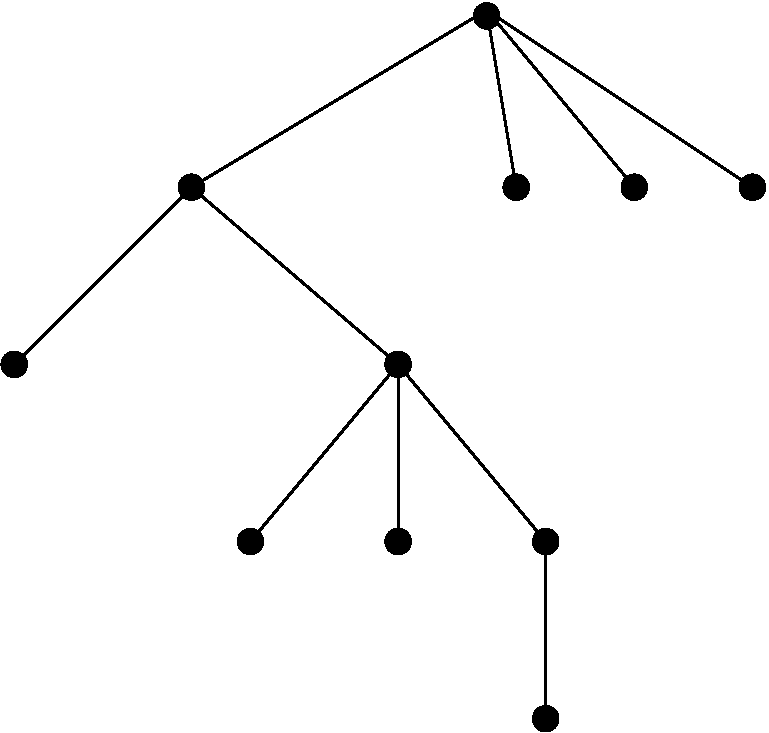
\includegraphics[scale=0.4]{figs/fig1.pdf}
      \quad \quad \quad \quad
    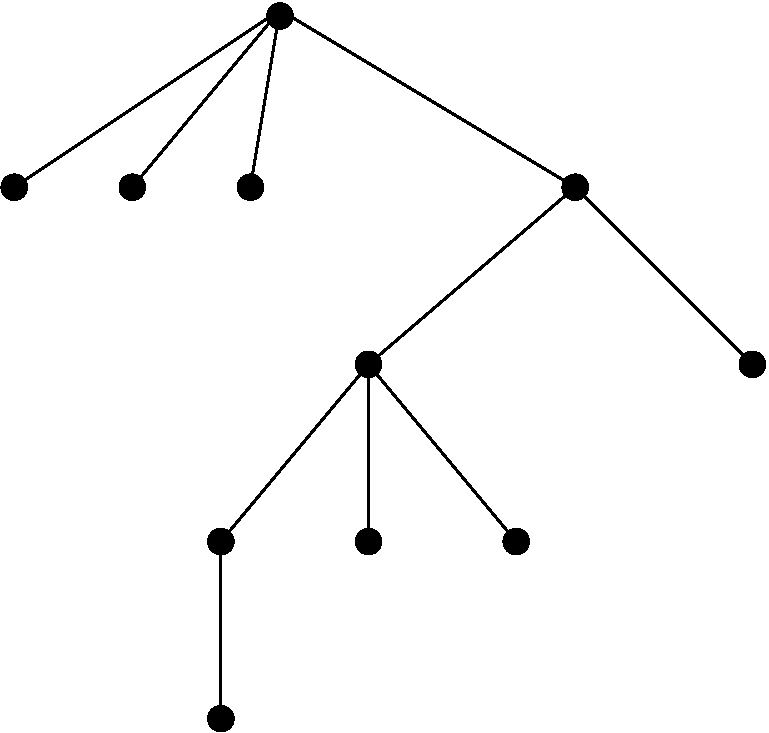
\includegraphics[scale=0.4]{figs/fig2.pdf}
    \caption{Un albero. A sinistra ogni nodo dichiara il numero di figli, a destra il numero di discendenti.}
\end{figure}

Proponiamo due possibili modi di codificare un albero come una sequenza di numeri naturali. Il primo numero della sequenza è $1$ oppure $2$ a seconda che si utilizzi la prima oppure la seconda codifica, e specifica appunto la codifica scelta. Seguono poi tanti numeri naturali quanti sono i nodi dell'albero. 
Nella prima codifica, l'albero viene descritto dicendo quanti figli ha la radice (in questo caso, quattro) e poi descrivendo uno a uno, nell'ordine da sinistra a destra, i quattro sottoalberi. In questo modo, ad esempio, l'albero in figura sarebbe identificato dalla seguente sequenza:
\[
1\,\,\,4\,\,\,2\,\,\,0\,\,\,3\,\,\,0\,\,\,0\,\,\,1\,\,\,0\,\,\,0\,\,\,0\,\,\,0
\]	

Infatti, l'albero ha quattro figli sotto la radice, per cui il primo numero dopo lo specificatore di formato ($1$) \`e $4$. A questo $4$ segue poi subito la sequenza $2\,\,\,0\,\,\,3\,\,\,0\,\,\,0\,\,\,1\,\,\,0$, che \`e la descrizione del primo figlio, mentre gli ultimi tre figli sono ciascuno descritti da $0$ (dato che non hanno figli).

Nella seconda codifica, i nodi dell'albero parlano nello stesso ordine, ma questa volta ciascuno scrive la numerosità dell'intera sua discendenza invece che limitarsi a dichiarare il numero dei propri figli.
Nella seconda codifica la sequenza generata dall'albero in figura è la seguente:
\[
2\,\,\,11\,\,\,7\,\,\,1\,\,\,5\,\,\,1\,\,\,1\,\,\,2\,\,\,1\,\,\,1\,\,\,1\,\,\,1
\]	


% Input
\section*{Dati di input}

Il vostro programma legge da \verb'input.txt' una sola riga contenente la codifica di un albero offerta secondo il primo o secondo formato.

% Output
\section*{Dati di output}

Il vostro programma deve restituire su \verb'output.txt' una sola riga,
la codifica dello stesso albero nell'altro formato.

% Esempi
\section*{Esempio di input/output}
\esempio{
1 4 2 0 3 0 0 1 0 0 0 0
}{
2 11 7 1 5 1 1 2 1 1 1 1
}

\section*{Esempio di input/output}
\esempio{
2 11 7 1 5 1 1 2 1 1 1 1
}{
1 4 2 0 3 0 0 1 0 0 0 0
}

% Assunzioni
\section*{Assunzioni}
\begin{itemize}[nolistsep, noitemsep]
\item dove $n$ \`e il numero di nodi dell'albero,
      vale sempre che $1 \le n \le 1\,000\,000 $;
\item tempo limite: un secondo.
\end{itemize}

% Subtasks
\section*{Subtask}
Alcune istanze ($x=0$) chiedono di passare dalla prima alla seconda codifica,
altre ($x=1$) chiedono di passare dalla seconda alla prima codifica.
\begin{itemize}
\item \textbf{Subtask 1 [0 punti]:} l'esempio del testo.
\item \textbf{Subtask x+2 [10 punti]:} ogni nodo ha massimo un figlio.
\item \textbf{Subtask x+3 [10 punti]:} ogni nodo ha massimo due figli.
\item \textbf{Subtask x+4 [10 punti]:} $N \le 10$.
\item \textbf{Subtask x+5 [10 punti]:} $N \le 1000$.
\item \textbf{Subtask x+6 [10 punti]:} $N \le 1\,000\,000$.
\end{itemize}


\end{document}
